\documentclass[11pt, landscape]{article}

\newcommand{\shellcmd}[1]{\texttt{\footnotesize #1}}

\usepackage{amsmath}
\usepackage{amsthm}
\usepackage{graphicx}
\usepackage{mathtools}
\usepackage{fullpage}
\usepackage{verbatim}

\allowdisplaybreaks

\title{Brownian Dynein Model}

\newcommand{\mn}{\scalebox{0.7}[1.0]{-}}

\begin{document}

\maketitle

\section{Cartesian from Angular Coordinates}
This section lays out the definitions of the coordinates of the Dynein model. \\
\begin{align}
  X_{bb} &= 0 \\
  X_{bm} &= X_{bb}+L_{s}\cos(\Theta_{bb}) \\
  X_{t}  &= X_{bm}+L_{t}\cos(\Theta_{bm}) \\
  X_{fm} &= X_{t} - L_{t}\cos(\Theta_{fm}) \\
  X_{fb} &= X_{fm} - L_{s}\cos(\Theta_{fb})
\end{align}

\begin{align}
  Y_{bb} &= 0 \\
  Y_{bm} &= Y_{bb}+L_{s}\sin(\Theta_{bb}) \\
  Y_{t}  &= Y_{bm}+L_{t}\sin(\Theta_{bm}) \\
  Y_{fm} &= Y_{t} - L_{t}\sin(\Theta_{fm}) \\
  Y_{fb} &= Y_{fm} - L_{s}\sin(\Theta_{fb})
\end{align}

\section{Cartesian Velocities}
This section shows the velocity definitions. \\
\begin{align}
  \dot{X}_{bb} &= 0 \\
  \dot{X}_{bm} &= \dot{X}_{bb} - L_{s}\sin(\Theta_{bb})\dot{\Theta}_{bb} \\
  \dot{X}_{t } &= \dot{X}_{bm} - L_{t}\sin(\Theta_{bm})\dot{\Theta}_{bm} \\
  \dot{X}_{fm} &= \dot{X}_{t } + L_{t}\sin(\Theta_{fm})\dot{\Theta}_{fm} \\
  \dot{X}_{fb} &= \dot{X}_{fm} + L_{s}\sin(\Theta_{fb})\dot{\Theta}_{fb}
\end{align}  
             
\begin{align}                                                                          
  \dot{Y}_{bb} &= 0 \\                                                        
  \dot{Y}_{bm} &= \dot{Y}_{bb} + L_{s}\cos(\Theta_{bb})\dot{\Theta}_{bb} \\
  \dot{Y}_{t}  &= \dot{Y}_{bm} + L_{t}\cos(\Theta_{bm})\dot{\Theta}_{bm} \\
  \dot{Y}_{fm} &= \dot{Y}_{t } - L_{t}\cos(\Theta_{fm})\dot{\Theta}_{fm} \\
  \dot{Y}_{fb} &= \dot{Y}_{fm} - L_{s}\cos(\Theta_{fb})\dot{\Theta}_{fb}
\end{align}


\section{Cartesian Velocities (expanded)}
This section expands the above definitions. \\
\begin{align}
  \dot{X}_{bb} &= 0 \\
  \dot{X}_{bm} &= - L_{s}\sin(\Theta_{bb})\dot{\Theta}_{bb} \\
  \dot{X}_{t } &= - L_{s}\sin(\Theta_{bb})\dot{\Theta}_{bb} - L_{t}\sin(\Theta_{bm})\dot{\Theta}_{bm} \\
  \dot{X}_{fm} &= - L_{s}\sin(\Theta_{bb})\dot{\Theta}_{bb} - L_{t}\sin(\Theta_{bm})\dot{\Theta}_{bm} + L_{t}\sin(\Theta_{fm})\dot{\Theta}_{fm} \\
  \dot{X}_{fb} &= - L_{s}\sin(\Theta_{bb})\dot{\Theta}_{bb} - L_{t}\sin(\Theta_{bm})\dot{\Theta}_{bm} + L_{t}\sin(\Theta_{fm})\dot{\Theta}_{fm} + L_{s}\sin(\Theta_{fb})\dot{\Theta}_{fb}
\end{align}             
             
\begin{align}                                                                               
  \dot{Y}_{bb} &= 0 \\                                                               
  \dot{Y}_{bm} &= L_{s}\cos(\Theta_{bb})\dot{\Theta}_{bb} \\
  \dot{Y}_{t}  &= L_{s}\cos(\Theta_{bb})\dot{\Theta}_{bb} + L_{t}\cos(\Theta_{bm})\dot{\Theta}_{bm} \\
  \dot{Y}_{fm} &= L_{s}\cos(\Theta_{bb})\dot{\Theta}_{bb} + L_{t}\cos(\Theta_{bm})\dot{\Theta}_{bm} - L_{t}\cos(\Theta_{fm})\dot{\Theta}_{fm} \\
  \dot{Y}_{fb} &= L_{s}\cos(\Theta_{bb})\dot{\Theta}_{bb} + L_{t}\cos(\Theta_{bm})\dot{\Theta}_{bm} - L_{t}\cos(\Theta_{fm})\dot{\Theta}_{fm} - L_{s}\cos(\Theta_{fb})\dot{\Theta}_{fb}
\end{align}


\section{Brownian Equations}
This section shows the velocity definitions using the Brownian dynamics equation. \\
\begin{align}  
  \dot{X}_{bb} &= 0 \\
  \dot{X}_{bm} &= \frac{1}{\gamma} \Big(F_{xml} + \mn \lambda_{bs}(X_{bm} - X_{bb}) + \lambda_{bt}(X_{t } - X_{bm}) \Big) + R_{xml} \\
  \dot{X}_{t } &= \frac{1}{\gamma} \Big(F_{xt } + \mn \lambda_{bt}(X_{t } - X_{bm}) + \lambda_{ft}(X_{fm} - X_{t }) \Big) + R_{xt } \\
  \dot{X}_{fm} &= \frac{1}{\gamma} \Big(F_{xmr} + \mn \lambda_{ft}(X_{fm} - X_{t }) + \lambda_{fs}(X_{fb} - X_{fm}) \Big) + R_{xmr} \\
  \dot{X}_{fb} &= \frac{1}{\gamma} \Big(F_{xbr} + \mn \lambda_{fs}(X_{fb} - X_{fm})                                 \Big) + R_{xbr}
\end{align}

\begin{align}  
  \dot{Y}_{bb} &= 0 \\
  \dot{Y}_{bm} &= \frac{1}{\gamma} \Big(F_{yml} + \mn \lambda_{bs}(Y_{bm} - Y_{bb}) + \lambda_{bt}(Y_{t } - Y_{bm}) \Big) + R_{yml} \\
  \dot{Y}_{t}  &= \frac{1}{\gamma} \Big(F_{yt } + \mn \lambda_{bt}(Y_{t } - Y_{bm}) + \lambda_{ft}(Y_{fm} - Y_{t }) \Big) + R_{yt } \\
  \dot{Y}_{fm} &= \frac{1}{\gamma} \Big(F_{ymr} + \mn \lambda_{ft}(Y_{fm} - Y_{t }) + \lambda_{fs}(Y_{fb} - Y_{fm}) \Big) + R_{ymr} \\
  \dot{Y}_{fb} &= \frac{1}{\gamma} \Big(F_{ybr} + \mn \lambda_{fs}(Y_{fb} - Y_{fm})                                 \Big) + R_{ybr}
\end{align}

%Unnecessary section commented out
\begin{comment}
\section{Expanded Brownian Equations}

\begin{align}
  &L_{s}\sin(\Theta_{bb})  \dot{\Theta}_{bb} = \frac{1}{\gamma}F_{xml} + \mn\frac{1}{\gamma}\lambda_{bs}(X_{bm} - X_{bb}) + \frac{1}{\gamma}\lambda_{bt}(X_{t } - X_{bm}) + R_{xml} \\
  &L_{s}\sin(\Theta_{bb})  \dot{\Theta}_{bb} + L_{t}\sin(\Theta_{bm})      \dot{\Theta}_{bm} = \frac{1}{\gamma}F_{xt } + \mn\frac{1}{\gamma}\lambda_{bt}(X_{t } - X_{bm}) + \frac{1}{\gamma}\lambda_{ft}(X_{fm} - X_{t }) + R_{xt } \\
  &L_{s}\sin(\Theta_{bb})  \dot{\Theta}_{bb} + L_{t}\sin(\Theta_{bm})      \dot{\Theta}_{bm} + L_{t}\sin(\Theta_{fm}-\pi)  \dot{\Theta}_{fm} = \frac{1}{\gamma}F_{xmr} + \mn\frac{1}{\gamma}\lambda_{ft}(X_{fm} - X_{t }) + \frac{1}{\gamma}\lambda_{fs}(X_{fb} - X_{fm}) + R_{xmr} \\
  &L_{s}\sin(\Theta_{bb})  \dot{\Theta}_{bb} + L_{t}\sin(\Theta_{bm})      \dot{\Theta}_{bm} + L_{t}\sin(\Theta_{fm}-\pi)  \dot{\Theta}_{fm} + L_{s}\sin(\Theta_{fb}-\pi)  \dot{\Theta}_{fb} = \frac{1}{\gamma}F_{xbr} + \mn\frac{1}{\gamma}\lambda_{fs}(X_{fb} - X_{fm}) + R_{xbr}
\end{align}

\begin{align}
  &\mn L_{s}\cos(\Theta_{bb})  \dot{\Theta}_{bb} = \frac{1}{\gamma}F_{yml} + \mn \frac{1}{\gamma}\lambda_{bs}(Y_{bm} - Y_{bb}) + \frac{1}{\gamma}\lambda_{bt}(Y_{t } - Y_{bm}) + R_{yml} \\
  &\mn L_{s}\cos(\Theta_{bb})  \dot{\Theta}_{bb} + \mn L_{t}\cos(\Theta_{bm})  \dot{\Theta}_{bm}  = \frac{1}{\gamma}F_{yt } + \mn \frac{1}{\gamma}\lambda_{bt}(Y_{t } - Y_{bm}) + \frac{1}{\gamma}\lambda_{ft}(Y_{fm} - Y_{t }) + R_{yt } \\
  &\mn L_{s}\cos(\Theta_{bb})  \dot{\Theta}_{bb} + \mn L_{t}\cos(\Theta_{bm})  \dot{\Theta}_{bm} + \mn L_{t}\cos(\Theta_{fm}-\pi)  \dot{\Theta}_{fm} = \frac{1}{\gamma}F_{ymr} + \mn \frac{1}{\gamma}\lambda_{ft}(Y_{fm} - Y_{t }) + \frac{1}{\gamma}\lambda_{fs}(Y_{fb} - Y_{fm}) + R_{ymr} \\
  &\mn L_{s}\cos(\Theta_{bb})  \dot{\Theta}_{bb} + \mn L_{t}\cos(\Theta_{bm})  \dot{\Theta}_{bm} + \mn L_{t}\cos(\Theta_{fm}-\pi)  \dot{\Theta}_{fm} + \mn L_{s}\cos(\Theta_{fb}-\pi)  \dot{\Theta}_{fb} = \frac{1}{\gamma}F_{ybr} + \mn \frac{1}{\gamma}\lambda_{fs}(Y_{fb} - Y_{fm}) + R_{ybr}
\end{align}


\section{System after Subtracting out Angular Velocity Terms}
This is the system after subtracting equations from each other to eliminate some angular velocity terms.\\

\begin{align}
  L_{s}\sin(\Theta_{bb})      \dot{\Theta}_{bb} &= \frac{1}{\gamma}F_{xml} - \frac{1}{\gamma}\lambda_{bs}(X_{bm} - X_{bb}) + \frac{1}{\gamma}\lambda_{bt}(X_{t } - X_{bm}) + R_{xml} \\
  L_{t}\sin(\Theta_{bm})      \dot{\Theta}_{bm} &= \frac{1}{\gamma}F_{xt } - \frac{2}{\gamma}\lambda_{bt}(X_{t } - X_{bm}) + \frac{1}{\gamma}\lambda_{ft}(X_{fm} - X_{t }) + R_{xt } - \frac{1}{\gamma}F_{xml} - \mn\frac{1}{\gamma}\lambda_{bs}(X_{bm} - X_{bb}) - R_{xml} \\
  L_{t}\sin(\Theta_{fm}-\pi)  \dot{\Theta}_{fm} &= \frac{1}{\gamma}F_{xmr} - \frac{2}{\gamma}\lambda_{ft}(X_{fm} - X_{t }) + \frac{1}{\gamma}\lambda_{fs}(X_{fb} - X_{fm}) + R_{xmr} - \frac{1}{\gamma}F_{xt } - \mn\frac{1}{\gamma}\lambda_{bt}(X_{t } - X_{bm}) - R_{xt } \\
  L_{s}\sin(\Theta_{fb}-\pi)  \dot{\Theta}_{fb} &= \frac{1}{\gamma}F_{xbr} - \frac{2}{\gamma}\lambda_{fs}(X_{fb} - X_{fm}) + R_{xbr} - \frac{1}{\gamma}F_{xmr} - \mn\frac{1}{\gamma}\lambda_{ft}(X_{fm} - X_{t }) - R_{xmr} 
\end{align}

\begin{align}
  \mn L_{s}\cos(\Theta_{bb})      \dot{\Theta}_{bb} &= \frac{1}{\gamma}F_{yml} - \frac{1}{\gamma}\lambda_{bs}(Y_{bm} - Y_{bb}) + \frac{1}{\gamma}\lambda_{bt}(Y_{t } - Y_{bm}) + R_{yml} \\
  \mn L_{t}\cos(\Theta_{bm})      \dot{\Theta}_{bm} &= \frac{1}{\gamma}F_{yt } - \frac{2}{\gamma}\lambda_{bt}(Y_{t } - Y_{bm}) + \frac{1}{\gamma}\lambda_{ft}(Y_{fm} - Y_{t }) + R_{yt } - \frac{1}{\gamma}F_{yml} - \mn \frac{1}{\gamma}\lambda_{bs}(Y_{bm} - Y_{bb}) - R_{yml}\\
  \mn L_{t}\cos(\Theta_{fm}-\pi)  \dot{\Theta}_{fm} &= \frac{1}{\gamma}F_{ymr} - \frac{2}{\gamma}\lambda_{ft}(Y_{fm} - Y_{t }) + \frac{1}{\gamma}\lambda_{fs}(Y_{fb} - Y_{fm}) + R_{ymr} - \frac{1}{\gamma}F_{yt } - \mn \frac{1}{\gamma}\lambda_{bt}(Y_{t } - Y_{bm}) - R_{yt } \\
  \mn L_{s}\cos(\Theta_{fb}-\pi)  \dot{\Theta}_{fb} &= \frac{1}{\gamma}F_{ybr} - \frac{2}{\gamma}\lambda_{fs}(Y_{fb} - Y_{fm}) + R_{ybr} - \frac{1}{\gamma}F_{ymr} - \mn \frac{1}{\gamma}\lambda_{ft}(Y_{fm} - Y_{t }) - R_{ymr} 
\end{align}
\end{comment}
  
\section{System of Equations}
This section creates a system of equations by equating the Cartesian and Brownian velocity definitions from above. \\

\begin{align}  
  \dot{X}_{bm} &= \dot{X}_{bb} + \mn L_{s}\sin(\Theta_{bb})\dot{\Theta}_{bb} = \frac{1}{\gamma}F_{xml} + \mn\frac{1}{\gamma}\lambda_{bs}(X_{bm} - X_{bb}) + \frac{1}{\gamma}\lambda_{bt}(X_{t } - X_{bm}) + R_{xml} \\
  \dot{X}_{t}  &= \dot{X}_{bm} + \mn L_{t}\sin(\Theta_{bm})\dot{\Theta}_{bm} = \frac{1}{\gamma}F_{xt } + \mn\frac{1}{\gamma}\lambda_{bt}(X_{t } - X_{bm}) + \frac{1}{\gamma}\lambda_{ft}(X_{fm} - X_{t }) + R_{xt } \\
  \dot{X}_{fm} &= \dot{X}_{t } + L_{t}\sin(\Theta_{fm})\dot{\Theta}_{fm} = \frac{1}{\gamma}F_{xmr} + \mn\frac{1}{\gamma}\lambda_{ft}(X_{fm} - X_{t }) + \frac{1}{\gamma}\lambda_{fs}(X_{fb} - X_{fm}) + R_{xmr} \\
  \dot{X}_{fb} &= \dot{X}_{fm} + L_{s}\sin(\Theta_{fb})\dot{\Theta}_{fb} = \frac{1}{\gamma}F_{xbr} + \mn\frac{1}{\gamma}\lambda_{fs}(X_{fb} - X_{fm}) + R_{xbr}
\end{align}

\begin{align}  
  \dot{Y}_{bm} &= \dot{Y}_{bb} + L_{s}\cos(\Theta_{bb})\dot{\Theta}_{bb} = \frac{1}{\gamma}F_{yml} + \mn\frac{1}{\gamma}\lambda_{bs}(Y_{bm} - Y_{bb}) + \frac{1}{\gamma}\lambda_{bt}(Y_{t } - Y_{bm}) + R_{yml} \\
  \dot{Y}_{t}  &= \dot{Y}_{bm} + L_{t}\cos(\Theta_{bm})\dot{\Theta}_{bm} = \frac{1}{\gamma}F_{yt } + \mn\frac{1}{\gamma}\lambda_{bt}(Y_{t } - Y_{bm}) + \frac{1}{\gamma}\lambda_{ft}(Y_{fm} - Y_{t }) + R_{yt } \\
  \dot{Y}_{fm} &= \dot{Y}_{t } + \mn L_{t}\cos(\Theta_{fm})\dot{\Theta}_{fm} = \frac{1}{\gamma}F_{ymr} + \mn\frac{1}{\gamma}\lambda_{ft}(Y_{fm} - Y_{t }) + \frac{1}{\gamma}\lambda_{fs}(Y_{fb} - Y_{fm}) + R_{ymr} \\
  \dot{Y}_{fb} &= \dot{Y}_{fm} + \mn L_{s}\cos(\Theta_{fb})\dot{\Theta}_{fb} = \frac{1}{\gamma}F_{ybr} + \mn\frac{1}{\gamma}\lambda_{fs}(Y_{fb} - Y_{fm}) + R_{ybr}
\end{align}

\section{System after Addition}
By adding equations from our system together we can isolate the $\lambda$ values. This system has been verified via CAS.\\

\begin{multline}
\mn\frac{1}{\gamma}\lambda_{bs}(X_{bm} - X_{bb}) =
\dot{X}_{bb} + \mn L_{s}\sin(\Theta_{bb})\dot{\Theta}_{bb} - R_{xml} - \frac{1}{\gamma}F_{xml} + \dot{X}_{bm} + \mn L_{t}\sin(\Theta_{bm})\dot{\Theta}_{bm} - R_{xt } \\
- \frac{1}{\gamma}F_{xt } + \dot{X}_{t } + L_{t}\sin(\Theta_{fm})\dot{\Theta}_{fm} - R_{xmr}
-\frac{1}{\gamma}F_{xmr} + \dot{X}_{fm} + L_{s}\sin(\Theta_{fb})\dot{\Theta}_{fb} - R_{xbr} - \frac{1}{\gamma}F_{xbr}
\label{eq:Ax}
\end{multline}%Fix'd

\begin{multline}
\mn\frac{1}{\gamma}\lambda_{bt}(X_{t } - X_{bm}) =
\dot{X}_{bm} + \mn L_{t}\sin(\Theta_{bm})\dot{\Theta}_{bm} - R_{xt } - \frac{1}{\gamma}F_{xt } + \dot{X}_{t } + L_{t}\sin(\Theta_{fm})\dot{\Theta}_{fm} \\
- R_{xmr} - \frac{1}{\gamma}F_{xmr} + \dot{X}_{fm} + L_{s}\sin(\Theta_{fb})\dot{\Theta}_{fb} - R_{xbr} - \frac{1}{\gamma}F_{xbr}
\label{eq:Bx}
\end{multline}%Fix'd

\begin{equation}
\mn\frac{1}{\gamma}\lambda_{ft}(X_{fm} - X_{t }) =
\dot{X}_{t } + L_{t}\sin(\Theta_{fm})\dot{\Theta}_{fm} - R_{xmr} - \frac{1}{\gamma}F_{xmr}
+ \dot{X}_{fm} + L_{s}\sin(\Theta_{fb})\dot{\Theta}_{fb} - R_{xbr} - \frac{1}{\gamma}F_{xbr}
\label{eq:Cx}
\end{equation}%Fix'd

\begin{equation}
\mn\frac{1}{\gamma}\lambda_{fs}(X_{fb} - X_{fm}) = 
\dot{X}_{fm} + L_{s}\sin(\Theta_{fb})\dot{\Theta}_{fb} - R_{xbr} - \frac{1}{\gamma}F_{xbr}
\label{eq:Dx}
\end{equation}%Fix'd


\begin{multline}
\mn\frac{1}{\gamma}\lambda_{bs}(Y_{bm} - Y_{bb}) =
\dot{Y}_{bb} + L_{s}\cos(\Theta_{bb})\dot{\Theta}_{bb} - R_{yml} - \frac{1}{\gamma}F_{yml} + \dot{Y}_{bm} + L_{t}\cos(\Theta_{bm})\dot{\Theta}_{bm} \\
- R_{yt} - \frac{1}{\gamma}F_{yt } + \dot{Y}_{t } + \mn L_{t}\cos(\Theta_{fm})\dot{\Theta}_{fm} - R_{ymr} - \frac{1}{\gamma}F_{ymr} + \dot{Y}_{fm}
+ \mn L_{s}\cos(\Theta_{fb})\dot{\Theta}_{fb} - R_{ybr} - \frac{1}{\gamma}F_{ybr}
\label{eq:Ay}
\end{multline}%Fix'd

\begin{multline}
\mn\frac{1}{\gamma}\lambda_{bt}(Y_{t } - Y_{bm}) =
\dot{Y}_{bm} + L_{t}\cos(\Theta_{bm})\dot{\Theta}_{bm} - R_{yt} - \frac{1}{\gamma}F_{yt } + \dot{Y}_{t } + \mn L_{t}\cos(\Theta_{fm})\dot{\Theta}_{fm} \\
- R_{ymr} - \frac{1}{\gamma}F_{ymr} + \dot{Y}_{fm} + \mn L_{s}\cos(\Theta_{fb})\dot{\Theta}_{fb} - R_{ybr} - \frac{1}{\gamma}F_{ybr}
\label{eq:By}
\end{multline}%Fix'd

\begin{equation}
\mn\frac{1}{\gamma}\lambda_{ft}(Y_{fm} - Y_{t }) =
\dot{Y}_{t } + \mn L_{t}\cos(\Theta_{fm})\dot{\Theta}_{fm} - R_{ymr} - \frac{1}{\gamma}F_{ymr} + \dot{Y}_{fm} + \mn L_{s}\cos(\Theta_{fb})\dot{\Theta}_{fb}
- R_{ybr} - \frac{1}{\gamma}F_{ybr}
\label{eq:Cy}
\end{equation}%Fix'd

\begin{equation}
\mn\frac{1}{\gamma}\lambda_{fs}(Y_{fb} - Y_{fm}) = \dot{Y}_{fm} + \mn L_{s}\cos(\Theta_{fb})\dot{\Theta}_{fb} - R_{ybr} - \frac{1}{\gamma}F_{ybr}
\label{eq:Dy}
\end{equation}%Fix'd

\section{Creating Angular Velocity Matrix}

Our goal is to take the above system of equations and put it in matrix form: 


\begin{align}
  A_1\dot{\Theta}_{bb} + A_2 \dot{\Theta}_{bm} + A_3 \dot{\Theta}_{fm} + A_4 \dot{\Theta}_{fb} &= X_1 \\
  B_1\dot{\Theta}_{bb} + B_2 \dot{\Theta}_{bm} + B_3 \dot{\Theta}_{fm} + B_4 \dot{\Theta}_{fb} &= X_2 \\
  C_1\dot{\Theta}_{bb} + C_2 \dot{\Theta}_{bm} + C_3 \dot{\Theta}_{fm} + C_4 \dot{\Theta}_{fb} &= X_3 \\
  D_1\dot{\Theta}_{bb} + D_2 \dot{\Theta}_{bm} + D_3 \dot{\Theta}_{fm} + D_4 \dot{\Theta}_{fb} &= X_4 \\
\end{align}

This will allow us to perform a matrix solution for the angular velocities. $X_1$, $X_2$, $X_3$ and $X_4$ contain only force terms and no unknown $\lambda$s. The above system of equations has four lambda terms: $\lambda_{bs}, \lambda_{bt}, \lambda_{ft}$ and $\lambda_{bs}$. Each term is present in two equations. We will use this redundancy to eliminate the lambda terms and create the above matrix.

\subsection{Solving for $A_1$, $A_2$, $A_3$, $A_4$ and $X_1$}
In this section we take Equations (\ref{eq:Ax}) and (\ref{eq:Ay}), equate them and manipulate them to be in form $A_1\dot{\Theta}_{bb} + A_2 \dot{\Theta}_{bm} + A_3 \dot{\Theta}_{fm} + A_4 \dot{\Theta}_{fb} = X_1$\\

We start by dividing out the position terms in Equations (\ref{eq:Ax}) and (\ref{eq:Ay}) to make their LHSs identical.

\begin{multline}
\mn\frac{1}{\gamma}\lambda_{bs} =
\Big(\dot{X}_{bb} + \mn L_{s}\sin(\Theta_{bb})\dot{\Theta}_{bb} - R_{xml} - \frac{1}{\gamma}F_{xml} + \dot{X}_{bm} + \mn L_{t}\sin(\Theta_{bm})\dot{\Theta}_{bm} - R_{xt } \\
- \frac{1}{\gamma}F_{xt } + \dot{X}_{t } + L_{t}\sin(\Theta_{fm})\dot{\Theta}_{fm} - R_{xmr}
-\frac{1}{\gamma}F_{xmr} + \dot{X}_{fm} + L_{s}\sin(\Theta_{fb})\dot{\Theta}_{fb} - R_{xbr} - \frac{1}{\gamma}F_{xbr}\Big)\frac{1}{(X_{bm} - X_{bb})}
\end{multline}

\begin{multline}
\mn\frac{1}{\gamma}\lambda_{bs} =
\Big( \dot{Y}_{bb} + L_{s}\cos(\Theta_{bb})\dot{\Theta}_{bb} - R_{yml} - \frac{1}{\gamma}F_{yml} + \dot{Y}_{bm} + L_{t}\cos(\Theta_{bm})\dot{\Theta}_{bm} \\
- R_{yt} - \frac{1}{\gamma}F_{yt } + \dot{Y}_{t } + \mn L_{t}\cos(\Theta_{fm})\dot{\Theta}_{fm} - R_{ymr} - \frac{1}{\gamma}F_{ymr} + \dot{Y}_{fm}
+ \mn L_{s}\cos(\Theta_{fb})\dot{\Theta}_{fb} - R_{ybr} - \frac{1}{\gamma}F_{ybr}\Big)\frac{1}{(Y_{bm} - Y_{bb})}
\end{multline}

We then equate them.

\begin{multline}
\Big(\dot{X}_{bb} + \mn L_{s}\sin(\Theta_{bb})\dot{\Theta}_{bb} - R_{xml} - \frac{1}{\gamma}F_{xml} + \dot{X}_{bm} + \mn L_{t}\sin(\Theta_{bm})\dot{\Theta}_{bm} - R_{xt } \\
- \frac{1}{\gamma}F_{xt } + \dot{X}_{t } + L_{t}\sin(\Theta_{fm})\dot{\Theta}_{fm} - R_{xmr}
-\frac{1}{\gamma}F_{xmr} + \dot{X}_{fm} + L_{s}\sin(\Theta_{fb})\dot{\Theta}_{fb} - R_{xbr} - \frac{1}{\gamma}F_{xbr}\Big)(Y_{bm} - Y_{bb}) = \\
\Big( \dot{Y}_{bb} + L_{s}\cos(\Theta_{bb})\dot{\Theta}_{bb} - R_{yml} - \frac{1}{\gamma}F_{yml} + \dot{Y}_{bm} + L_{t}\cos(\Theta_{bm})\dot{\Theta}_{bm}
- R_{yt} - \frac{1}{\gamma}F_{yt } + \dot{Y}_{t } + \mn L_{t}\cos(\Theta_{fm})\dot{\Theta}_{fm} - R_{ymr} - \frac{1}{\gamma}F_{ymr} + \dot{Y}_{fm} \\
+ \mn L_{s}\cos(\Theta_{fb})\dot{\Theta}_{fb} - R_{ybr} - \frac{1}{\gamma}F_{ybr}\Big)(X_{bm} - X_{bb})
\end{multline}

Then we group like terms for clarity.

\begin{multline}
\Big(\dot{X}_{bb} + \dot{X}_{bm} + \dot{X}_{t } + \dot{X}_{fm} 
- L_{s}\sin(\Theta_{bb})\dot{\Theta}_{bb} - L_{t}\sin(\Theta_{bm})\dot{\Theta}_{bm} + L_{t}\sin(\Theta_{fm})\dot{\Theta}_{fm} + L_{s}\sin(\Theta_{fb})\dot{\Theta}_{fb} \\
- \frac{1}{\gamma}F_{xml} - \frac{1}{\gamma}F_{xt } -\frac{1}{\gamma}F_{xmr} - \frac{1}{\gamma}F_{xbr}
- R_{xml} - R_{xt } - R_{xmr} - R_{xbr} \Big)(L_s\sin(\Theta_{bb})) = \\
\Big(\dot{Y}_{bb} + \dot{Y}_{bm} + \dot{Y}_{t } + \dot{Y}_{fm}
+ L_{s}\cos(\Theta_{bb})\dot{\Theta}_{bb} + L_{t}\cos(\Theta_{bm})\dot{\Theta}_{bm} - L_{t}\cos(\Theta_{fm})\dot{\Theta}_{fm} - L_{s}\cos(\Theta_{fb})\dot{\Theta}_{fb} \\
- \frac{1}{\gamma}F_{yml} - \frac{1}{\gamma}F_{yt } - \frac{1}{\gamma}F_{ymr} - \frac{1}{\gamma}F_{ybr}
- R_{yml} - R_{yt} - R_{ymr} - R_{ybr}\Big)(L_s\cos(\Theta_{bb}))
\end{multline}

We then expand all the $\dot{X}$ terms using their definitions from the Cartesian Velocities section above.

\begin{multline}
\Big(
- L_{s}\sin(\Theta_{bb})\dot{\Theta}_{bb}
- L_{s}\sin(\Theta_{bb})\dot{\Theta}_{bb} - L_{t}\sin(\Theta_{bm})\dot{\Theta}_{bm}
- L_{s}\sin(\Theta_{bb})\dot{\Theta}_{bb} - L_{t}\sin(\Theta_{bm})\dot{\Theta}_{bm} + L_{t}\sin(\Theta_{fm})\dot{\Theta}_{fm}\\
- L_{s}\sin(\Theta_{bb})\dot{\Theta}_{bb} - L_{t}\sin(\Theta_{bm})\dot{\Theta}_{bm} + L_{t}\sin(\Theta_{fm})\dot{\Theta}_{fm} + L_{s}\sin(\Theta_{fb})\dot{\Theta}_{fb}
- \frac{1}{\gamma}F_{xml} - \frac{1}{\gamma}F_{xt } -\frac{1}{\gamma}F_{xmr} - \frac{1}{\gamma}F_{xbr}
- R_{xml} - R_{xt } - R_{xmr} - R_{xbr} \Big)(L_s\sin(\Theta_{bb})) = \\
\Big(
+ L_{s}\cos(\Theta_{bb})\dot{\Theta}_{bb}
+ L_{s}\cos(\Theta_{bb})\dot{\Theta}_{bb} + L_{t}\cos(\Theta_{bm})\dot{\Theta}_{bm}
+ L_{s}\cos(\Theta_{bb})\dot{\Theta}_{bb} + L_{t}\cos(\Theta_{bm})\dot{\Theta}_{bm} - L_{t}\cos(\Theta_{fm})\dot{\Theta}_{fm}\\
+ L_{s}\cos(\Theta_{bb})\dot{\Theta}_{bb} + L_{t}\cos(\Theta_{bm})\dot{\Theta}_{bm} - L_{t}\cos(\Theta_{fm})\dot{\Theta}_{fm} - L_{s}\cos(\Theta_{fb})\dot{\Theta}_{fb}
- \frac{1}{\gamma}F_{yml} - \frac{1}{\gamma}F_{yt } - \frac{1}{\gamma}F_{ymr} - \frac{1}{\gamma}F_{ybr}
- R_{yml} - R_{yt} - R_{ymr} - R_{ybr}\Big)(L_s\cos(\Theta_{bb}))
\end{multline}

Then we group together the like terms from the expansion.

\begin{multline}
\Big(- 4L_{s}\sin(\Theta_{bb})\dot{\Theta}_{bb} - 3L_{t}\sin(\Theta_{bm})\dot{\Theta}_{bm} + 2L_{t}\sin(\Theta_{fm})\dot{\Theta}_{fm} + L_{s}\sin(\Theta_{fb})\dot{\Theta}_{fb}
- \frac{1}{\gamma}F_{xml} - \frac{1}{\gamma}F_{xt } -\frac{1}{\gamma}F_{xmr} - \frac{1}{\gamma}F_{xbr}
- R_{xml} - R_{xt } - R_{xmr} - R_{xbr} \Big)(L_s\sin(\Theta_{bb})) = \\
\Big(4L_{s}\cos(\Theta_{bb})\dot{\Theta}_{bb} + 3L_{t}\cos(\Theta_{bm})\dot{\Theta}_{bm} - 2L_{t}\cos(\Theta_{fm})\dot{\Theta}_{fm} - L_{s}\cos(\Theta_{fb})\dot{\Theta}_{fb}
- \frac{1}{\gamma}F_{yml} - \frac{1}{\gamma}F_{yt } - \frac{1}{\gamma}F_{ymr} - \frac{1}{\gamma}F_{ybr}
- R_{yml} - R_{yt} - R_{ymr} - R_{ybr}\Big)(L_s\cos(\Theta_{bb}))
\end{multline}

We then bring all the angular velocity terms to one side and all the force terms to the other side.

\begin{multline}
\Big(- 4L_{s}\sin(\Theta_{bb})\dot{\Theta}_{bb} - 3L_{t}\sin(\Theta_{bm})\dot{\Theta}_{bm}
+ 2L_{t}\sin(\Theta_{fm})\dot{\Theta}_{fm} + L_{s}\sin(\Theta_{fb})\dot{\Theta}_{fb}\Big)(L_s\sin(\Theta_{bb}))\\
\Big(-4L_{s}\cos(\Theta_{bb})\dot{\Theta}_{bb} - 3L_{t}\cos(\Theta_{bm})\dot{\Theta}_{bm}
+ 2L_{t}\cos(\Theta_{fm})\dot{\Theta}_{fm} + L_{s}\cos(\Theta_{fb})\dot{\Theta}_{fb}\Big)(L_s\cos(\Theta_{bb}))= \\
\Big(- \frac{1}{\gamma}F_{yml} - \frac{1}{\gamma}F_{yt } - \frac{1}{\gamma}F_{ymr} - \frac{1}{\gamma}F_{ybr} - R_{yml} - R_{yt} - R_{ymr} - R_{ybr}\Big)(L_s\cos(\Theta_{bb}))
+ \Big( \frac{1}{\gamma}F_{xml} + \frac{1}{\gamma}F_{xt } + \frac{1}{\gamma}F_{xmr} + \frac{1}{\gamma}F_{xbr} + R_{xml} + R_{xt } + R_{xmr} + R_{xbr} \Big)(L_s\sin(\Theta_{bb}))
\end{multline}

We then distribute the $L_s\sin(\Theta_{bb})$ and $L_s\cos(\Theta_{bb})$ terms into the expression.

\begin{multline}
\Big(- 4L_{s}\sin(\Theta_{bb})\sin(\Theta_{bb})\dot{\Theta}_{bb} - 3L_{t}\sin(\Theta_{bm})\sin(\Theta_{bb})\dot{\Theta}_{bm}
+ 2L_{t}\sin(\Theta_{fm})\sin(\Theta_{bb})\dot{\Theta}_{fm} + L_{s}\sin(\Theta_{fb})\sin(\Theta_{bb})\dot{\Theta}_{fb}\Big)\\
\Big(-4L_{s}\cos(\Theta_{bb})\cos(\Theta_{bb})\dot{\Theta}_{bb} - 3L_{t}\cos(\Theta_{bm})\cos(\Theta_{bb})\dot{\Theta}_{bm}
+ 2L_{t}\cos(\Theta_{fm})\cos(\Theta_{bb})\dot{\Theta}_{fm} + L_{s}\cos(\Theta_{fb})\cos(\Theta_{bb})\dot{\Theta}_{fb}\Big)= \\
\Big(- \frac{1}{\gamma}F_{yml} - \frac{1}{\gamma}F_{yt } - \frac{1}{\gamma}F_{ymr} - \frac{1}{\gamma}F_{ybr} - R_{yml} - R_{yt} - R_{ymr} - R_{ybr}\Big)(\cos(\Theta_{bb}))
+ \Big( \frac{1}{\gamma}F_{xml} + \frac{1}{\gamma}F_{xt } + \frac{1}{\gamma}F_{xmr} + \frac{1}{\gamma}F_{xbr} + R_{xml} + R_{xt } + R_{xmr} + R_{xbr} \Big)(\sin(\Theta_{bb}))
\end{multline}

Finally, we group all terms by their angular velocity.

\begin{multline}
-4L_{s}\Big(\sin(\Theta_{bb})\sin(\Theta_{bb}) + \cos(\Theta_{bb})\cos(\Theta_{bb})\Big)\dot{\Theta}_{bb}
-3L_{t}\Big(\sin(\Theta_{bm})\sin(\Theta_{bb}) + \cos(\Theta_{bm})\cos(\Theta_{bb})\Big)\dot{\Theta}_{bm}\\
+2L_{t}\Big(\sin(\Theta_{fm})\sin(\Theta_{bb}) + \cos(\Theta_{fm})\cos(\Theta_{bb})\Big)\dot{\Theta}_{fm}
+ L_{s}\Big(\sin(\Theta_{fb})\sin(\Theta_{bb}) + \cos(\Theta_{fb})\cos(\Theta_{bb})\Big)\dot{\Theta}_{fb}= \\
\Big(- \frac{1}{\gamma}F_{yml} - \frac{1}{\gamma}F_{yt } - \frac{1}{\gamma}F_{ymr} - \frac{1}{\gamma}F_{ybr} - R_{yml} - R_{yt} - R_{ymr} - R_{ybr}\Big)(\cos(\Theta_{bb}))
+ \Big( \frac{1}{\gamma}F_{xml} + \frac{1}{\gamma}F_{xt } + \frac{1}{\gamma}F_{xmr} + \frac{1}{\gamma}F_{xbr} + R_{xml} + R_{xt } + R_{xmr} + R_{xbr} \Big)(\sin(\Theta_{bb}))
\end{multline}

This is the form we want. We now know the value of $A_1, A_2, A_3, A_4$ and $X_1$.

\begin{align}
  A_1 &= -4L_{s}\\
  A_2 &= -3L_{t}\Big(\sin(\Theta_{bm})\sin(\Theta_{bb}) + \cos(\Theta_{bm})\cos(\Theta_{bb})\Big)\\
  A_3 &= 2L_{t}\Big(\sin(\Theta_{fm})\sin(\Theta_{bb}) + \cos(\Theta_{fm})\cos(\Theta_{bb})\Big)\\
  A_4 &= L_{s}\Big(\sin(\Theta_{fb})\sin(\Theta_{bb}) + \cos(\Theta_{fb})\cos(\Theta_{bb})\Big)\\
  X_1 &= \Big(- \frac{1}{\gamma}F_{yml} - \frac{1}{\gamma}F_{yt } - \frac{1}{\gamma}F_{ymr} - \frac{1}{\gamma}F_{ybr} - R_{yml} - R_{yt} - R_{ymr} - R_{ybr}\Big)(\cos(\Theta_{bb}))+\\
      &+ \Big( \frac{1}{\gamma}F_{xml} + \frac{1}{\gamma}F_{xt } + \frac{1}{\gamma}F_{xmr} + \frac{1}{\gamma}F_{xbr} + R_{xml} + R_{xt } + R_{xmr} + R_{xbr} \Big)(\sin(\Theta_{bb}))
\end{align}


\subsection{Solving for $B_1$, $B_2$, $B_3$, $B_4$ and $X_2$}
Here we take Equations (\ref{eq:Bx}) and (\ref{eq:By}), equate them and manipulate them to be in form $B_1\dot{\Theta}_{bb} + B_2 \dot{\Theta}_{bm} + B_3 \dot{\Theta}_{fm} + B_4 \dot{\Theta}_{fb} = X_2$

\begin{multline}
-\frac{1}{\gamma}\lambda_{bt} =
\Big(
\dot{X}_{bm} + \dot{X}_{t } + \dot{X}_{fm}
- L_{t}\sin(\Theta_{bm})\dot{\Theta}_{bm} + L_{t}\sin(\Theta_{fm})\dot{\Theta}_{fm} + L_{s}\sin(\Theta_{fb})\dot{\Theta}_{fb} 
- \frac{1}{\gamma}F_{xt } - \frac{1}{\gamma}F_{xmr} - \frac{1}{\gamma}F_{xbr}
- R_{xt } - R_{xmr} - R_{xbr}\Big) \frac{1}{(X_{t } - X_{bm})}
\end{multline}

\begin{multline}
-\frac{1}{\gamma}\lambda_{bt} =
\Big(
\dot{Y}_{bm} + \dot{Y}_{t } + \dot{Y}_{fm} 
+ L_{t}\cos(\Theta_{bm})\dot{\Theta}_{bm} - L_{t}\cos(\Theta_{fm})\dot{\Theta}_{fm} - L_{s}\cos(\Theta_{fb})\dot{\Theta}_{fb} 
- \frac{1}{\gamma}F_{yt } - \frac{1}{\gamma}F_{ymr} - \frac{1}{\gamma}F_{ybr}
- R_{yt} - R_{ymr} - R_{ybr}\Big) \frac{1}{(Y_{t } - Y_{bm})}
\end{multline}

\begin{multline}
\Big(
\dot{X}_{bm} + \dot{X}_{t } + \dot{X}_{fm}
- L_{t}\sin(\Theta_{bm})\dot{\Theta}_{bm} + L_{t}\sin(\Theta_{fm})\dot{\Theta}_{fm} + L_{s}\sin(\Theta_{fb})\dot{\Theta}_{fb} 
- \frac{1}{\gamma}F_{xt } - \frac{1}{\gamma}F_{xmr} - \frac{1}{\gamma}F_{xbr}
- R_{xt } - R_{xmr} - R_{xbr}\Big)(Y_{t } - Y_{bm}) =\\
\Big(
\dot{Y}_{bm} + \dot{Y}_{t } + \dot{Y}_{fm} 
+ L_{t}\cos(\Theta_{bm})\dot{\Theta}_{bm} - L_{t}\cos(\Theta_{fm})\dot{\Theta}_{fm} - L_{s}\cos(\Theta_{fb})\dot{\Theta}_{fb} 
- \frac{1}{\gamma}F_{yt } - \frac{1}{\gamma}F_{ymr} - \frac{1}{\gamma}F_{ybr}
- R_{yt} - R_{ymr} - R_{ybr}\Big)(X_{t } - X_{bm})
\end{multline}

\begin{multline}
\Big(
\dot{X}_{bm} + \dot{X}_{t } + \dot{X}_{fm}
- L_{t}\sin(\Theta_{bm})\dot{\Theta}_{bm} + L_{t}\sin(\Theta_{fm})\dot{\Theta}_{fm} + L_{s}\sin(\Theta_{fb})\dot{\Theta}_{fb} 
- \frac{1}{\gamma}F_{xt } - \frac{1}{\gamma}F_{xmr} - \frac{1}{\gamma}F_{xbr}
- R_{xt } - R_{xmr} - R_{xbr}\Big)(L_t\sin(\Theta_{bm})) =\\
\Big(
\dot{Y}_{bm} + \dot{Y}_{t } + \dot{Y}_{fm} 
+ L_{t}\cos(\Theta_{bm})\dot{\Theta}_{bm} - L_{t}\cos(\Theta_{fm})\dot{\Theta}_{fm} - L_{s}\cos(\Theta_{fb})\dot{\Theta}_{fb} 
- \frac{1}{\gamma}F_{yt } - \frac{1}{\gamma}F_{ymr} - \frac{1}{\gamma}F_{ybr}
- R_{yt} - R_{ymr} - R_{ybr}\Big)(L_t\cos(\Theta_{bm}))
\end{multline}

\begin{multline}
\Big(\dot{X}_{bm} + \dot{X}_{t } + \dot{X}_{fm}
- L_{t}\sin(\Theta_{bm})\dot{\Theta}_{bm} + L_{t}\sin(\Theta_{fm})\dot{\Theta}_{fm} + L_{s}\sin(\Theta_{fb})\dot{\Theta}_{fb}\Big)(L_t\sin(\Theta_{bm}))\\
- \Big(\dot{Y}_{bm} + \dot{Y}_{t } + \dot{Y}_{fm} 
+ L_{t}\cos(\Theta_{bm})\dot{\Theta}_{bm} - L_{t}\cos(\Theta_{fm})\dot{\Theta}_{fm} - L_{s}\cos(\Theta_{fb})\dot{\Theta}_{fb}\Big)(L_t\cos(\Theta_{bm})) =\\
\Big(-\frac{1}{\gamma}F_{yt } - \frac{1}{\gamma}F_{ymr} - \frac{1}{\gamma}F_{ybr} - R_{yt} - R_{ymr} - R_{ybr}\Big)(L_t\cos(\Theta_{bm}))
- \Big(-\frac{1}{\gamma}F_{xt } - \frac{1}{\gamma}F_{xmr} - \frac{1}{\gamma}F_{xbr} - R_{xt } - R_{xmr} - R_{xbr}\Big)(L_t\sin(\Theta_{bm}))
\end{multline}

\begin{multline}
\Big( -3L_{s}\sin(\Theta_{bb})\dot{\Theta}_{bb} - 3L_{t}\sin(\Theta_{bm})\dot{\Theta}_{bm} + 2L_{t}\sin(\Theta_{fm})\dot{\Theta}_{fm}
+ L_{s}\sin(\Theta_{fb})\dot{\Theta}_{fb}\Big)(L_t\sin(\Theta_{bm}))\\
- \Big( 3L_{s}\cos(\Theta_{bb})\dot{\Theta}_{bb} + 3L_{t}\cos(\Theta_{bm})\dot{\Theta}_{bm} -2L_{t}\cos(\Theta_{fm})\dot{\Theta}_{fm}
- L_{s}\cos(\Theta_{fb})\dot{\Theta}_{fb}\Big)(L_t\cos(\Theta_{bm})) =\\
\Big(-\frac{1}{\gamma}F_{yt } - \frac{1}{\gamma}F_{ymr} - \frac{1}{\gamma}F_{ybr} - R_{yt} - R_{ymr} - R_{ybr}\Big)(L_t\cos(\Theta_{bm}))
- \Big(-\frac{1}{\gamma}F_{xt } - \frac{1}{\gamma}F_{xmr} - \frac{1}{\gamma}F_{xbr} - R_{xt } - R_{xmr} - R_{xbr}\Big)(L_t\sin(\Theta_{bm}))
\end{multline}

\begin{multline}
\Big( -3L_{s}\sin(\Theta_{bb})\dot{\Theta}_{bb} - 3L_{t}\sin(\Theta_{bm})\dot{\Theta}_{bm} + 2L_{t}\sin(\Theta_{fm})\dot{\Theta}_{fm}
+ L_{s}\sin(\Theta_{fb})\dot{\Theta}_{fb}\Big)(L_t\sin(\Theta_{bm}))\\
+ \Big(-3L_{s}\cos(\Theta_{bb})\dot{\Theta}_{bb} - 3L_{t}\cos(\Theta_{bm})\dot{\Theta}_{bm} + 2L_{t}\cos(\Theta_{fm})\dot{\Theta}_{fm}
+ L_{s}\cos(\Theta_{fb})\dot{\Theta}_{fb}\Big)(L_t\cos(\Theta_{bm})) =\\
\Big(-\frac{1}{\gamma}F_{yt } - \frac{1}{\gamma}F_{ymr} - \frac{1}{\gamma}F_{ybr} - R_{yt} - R_{ymr} - R_{ybr}\Big)(L_t\cos(\Theta_{bm}))
+ \Big(\frac{1}{\gamma}F_{xt } + \frac{1}{\gamma}F_{xmr} + \frac{1}{\gamma}F_{xbr} + R_{xt } + R_{xmr} + R_{xbr}\Big)(L_t\sin(\Theta_{bm}))
\end{multline}

\begin{multline}
\Big( -3L_{s}\sin(\Theta_{bb})L_t\sin(\Theta_{bm})\dot{\Theta}_{bb} - 3L_{t}\sin(\Theta_{bm})L_t\sin(\Theta_{bm})\dot{\Theta}_{bm}
+ 2L_{t}\sin(\Theta_{fm})L_t\sin(\Theta_{bm})\dot{\Theta}_{fm} + L_{s}\sin(\Theta_{fb})L_t\sin(\Theta_{bm})\dot{\Theta}_{fb}\Big)\\
+ \Big(-3L_{s}\cos(\Theta_{bb})L_t\cos(\Theta_{bm})\dot{\Theta}_{bb} - 3L_{t}\cos(\Theta_{bm})L_t\cos(\Theta_{bm})\dot{\Theta}_{bm}
+ 2L_{t}\cos(\Theta_{fm})L_t\cos(\Theta_{bm})\dot{\Theta}_{fm} + L_{s}\cos(\Theta_{fb})L_t\cos(\Theta_{bm})\dot{\Theta}_{fb}\Big) =\\
\Big(-\frac{1}{\gamma}F_{yt } - \frac{1}{\gamma}F_{ymr} - \frac{1}{\gamma}F_{ybr} - R_{yt} - R_{ymr} - R_{ybr}\Big)(L_t\cos(\Theta_{bm}))
+ \Big(\frac{1}{\gamma}F_{xt } + \frac{1}{\gamma}F_{xmr} + \frac{1}{\gamma}F_{xbr} + R_{xt } + R_{xmr} + R_{xbr}\Big)(L_t\sin(\Theta_{bm}))
\end{multline}

\begin{multline}
-3L_{s}\Big(\sin(\Theta_{bb})\sin(\Theta_{bm}) + \cos(\Theta_{bb})\cos(\Theta_{bm})\Big)\dot{\Theta}_{bb}
-3L_{t}\Big(\sin(\Theta_{bm})\sin(\Theta_{bm}) + \cos(\Theta_{bm})\cos(\Theta_{bm})\Big)\dot{\Theta}_{bm}\\
+2L_{t}\Big(\sin(\Theta_{fm})\sin(\Theta_{bm}) + \cos(\Theta_{fm})\cos(\Theta_{bm})\Big)\dot{\Theta}_{fm}
+ L_{s}\Big(\sin(\Theta_{fb})\sin(\Theta_{bm}) + \cos(\Theta_{fb})\cos(\Theta_{bm})\Big)\dot{\Theta}_{fb} =\\
\Big(-\frac{1}{\gamma}F_{yt } - \frac{1}{\gamma}F_{ymr} - \frac{1}{\gamma}F_{ybr} - R_{yt} - R_{ymr} - R_{ybr}\Big)(\cos(\Theta_{bm}))
+ \Big(\frac{1}{\gamma}F_{xt } + \frac{1}{\gamma}F_{xmr} + \frac{1}{\gamma}F_{xbr} + R_{xt } + R_{xmr} + R_{xbr}\Big)(\sin(\Theta_{bm}))
\end{multline}

\begin{align}
  B_1 &= -3L_{s}\Big(\sin(\Theta_{bb})\sin(\Theta_{bm}) + \cos(\Theta_{bb})\cos(\Theta_{bm})\Big)\\
  B_2 &= -3L_{t}\\
  B_3 &= +2L_{t}\Big(\sin(\Theta_{fm})\sin(\Theta_{bm}) + \cos(\Theta_{fm})\cos(\Theta_{bm})\Big)\\
  B_4 &= + L_{s}\Big(\sin(\Theta_{fb})\sin(\Theta_{bm}) + \cos(\Theta_{fb})\cos(\Theta_{bm})\Big)\\
  X_2 &= \Big(-\frac{1}{\gamma}F_{yt } - \frac{1}{\gamma}F_{ymr} - \frac{1}{\gamma}F_{ybr} - R_{yt} - R_{ymr} - R_{ybr}\Big)(\cos(\Theta_{bm}))\\
      &+ \Big(\frac{1}{\gamma}F_{xt } + \frac{1}{\gamma}F_{xmr} + \frac{1}{\gamma}F_{xbr} + R_{xt } + R_{xmr} + R_{xbr}\Big)(\sin(\Theta_{bm}))
\end{align}


\subsection{Solving for $C_1$, $C_2$, $C_3$, $C_4$ and $X_3$}
Here we take Equations (\ref{eq:Cx}) and (\ref{eq:Cy}), equate them and manipulate them to be in form $ C_1\dot{\Theta}_{bb} + C_2 \dot{\Theta}_{bm} + C_3 \dot{\Theta}_{fm} + C_4 \dot{\Theta}_{fb} = X_3$

\begin{equation}
-\frac{1}{\gamma}\lambda_{ft} = \Big( \dot{X}_{t } + L_{t}\sin(\Theta_{fm})\dot{\Theta}_{fm} - R_{xmr} - \frac{1}{\gamma}F_{xmr}
+ \dot{X}_{fm} + L_{s}\sin(\Theta_{fb})\dot{\Theta}_{fb} - R_{xbr} - \frac{1}{\gamma}F_{xbr}\Big) \frac{1}{(X_{fm} - X_{t })}
\end{equation}

\begin{equation}
-\frac{1}{\gamma}\lambda_{ft} = \Big( \dot{Y}_{t } - L_{t}\cos(\Theta_{fm})\dot{\Theta}_{fm} - R_{ymr} - \frac{1}{\gamma}F_{ymr}
+ \dot{Y}_{fm} - L_{s}\cos(\Theta_{fb})\dot{\Theta}_{fb} - R_{ybr} - \frac{1}{\gamma}F_{ybr}\Big) \frac{1}{(Y_{fm} - Y_{t })}
\end{equation}

\begin{multline}
\Big( \dot{X}_{t } + L_{t}\sin(\Theta_{fm})\dot{\Theta}_{fm} - R_{xmr} - \frac{1}{\gamma}F_{xmr}
+ \dot{X}_{fm} + L_{s}\sin(\Theta_{fb})\dot{\Theta}_{fb} - R_{xbr} - \frac{1}{\gamma}F_{xbr}\Big)(-L_{t}\sin(\Theta_{fm})) = \\
\Big( \dot{Y}_{t } - L_{t}\cos(\Theta_{fm})\dot{\Theta}_{fm} - R_{ymr} - \frac{1}{\gamma}F_{ymr}
+ \dot{Y}_{fm} - L_{s}\cos(\Theta_{fb})\dot{\Theta}_{fb} - R_{ybr} - \frac{1}{\gamma}F_{ybr}\Big)(-L_{t}\cos(\Theta_{fm}))
\end{multline}

\begin{multline}
\Big( \dot{X}_{t } + \dot{X}_{fm} + L_{t}\sin(\Theta_{fm})\dot{\Theta}_{fm} + L_{s}\sin(\Theta_{fb})\dot{\Theta}_{fb} \Big)\sin(\Theta_{fm}) +
\Big(- R_{xmr} - \frac{1}{\gamma}F_{xmr} - R_{xbr} - \frac{1}{\gamma}F_{xbr}\Big)\sin(\Theta_{fm}) = \\
\Big(\dot{Y}_{t } + \dot{Y}_{fm} - L_{t}\cos(\Theta_{fm})\dot{\Theta}_{fm} - L_{s}\cos(\Theta_{fb})\dot{\Theta}_{fb}\Big)\cos(\Theta_{fm}) +
\Big(- R_{ymr} - \frac{1}{\gamma}F_{ymr} - R_{ybr} - \frac{1}{\gamma}F_{ybr}\Big)\cos(\Theta_{fm})
\end{multline}

\begin{multline}
\Big( \dot{X}_{t } + \dot{X}_{fm} + L_{t}\sin(\Theta_{fm})\dot{\Theta}_{fm} + L_{s}\sin(\Theta_{fb})\dot{\Theta}_{fb} \Big)\sin(\Theta_{fm})
+ \Big(-\dot{Y}_{t } - \dot{Y}_{fm} + L_{t}\cos(\Theta_{fm})\dot{\Theta}_{fm} + L_{s}\cos(\Theta_{fb})\dot{\Theta}_{fb}\Big)\cos(\Theta_{fm}) = \\
\Big(- R_{ymr} - \frac{1}{\gamma}F_{ymr} - R_{ybr} - \frac{1}{\gamma}F_{ybr}\Big)\cos(\Theta_{fm})
+ \Big(R_{xmr} + \frac{1}{\gamma}F_{xmr} + R_{xbr} + \frac{1}{\gamma}F_{xbr}\Big)\sin(\Theta_{fm})
\end{multline}

\begin{multline}
\Big(- L_{s}\sin(\Theta_{bb})\dot{\Theta}_{bb} - L_{t}\sin(\Theta_{bm})\dot{\Theta}_{bm} + -L_{s}\sin(\Theta_{bb})\dot{\Theta}_{bb} - L_{t}\sin(\Theta_{bm})\dot{\Theta}_{bm} +
L_{t}\sin(\Theta_{fm})\dot{\Theta}_{fm} + L_{t}\sin(\Theta_{fm})\dot{\Theta}_{fm} +L_{s}\sin(\Theta_{fb})\dot{\Theta}_{fb} \Big)\sin(\Theta_{fm}) \\
+ \Big(-(L_{s}\cos(\Theta_{bb})\dot{\Theta}_{bb} + L_{t}\cos(\Theta_{bm})\dot{\Theta}_{bm}) -(L_{s}\cos(\Theta_{bb})\dot{\Theta}_{bb} + L_{t}\cos(\Theta_{bm})\dot{\Theta}_{bm} -
L_{t}\cos(\Theta_{fm})\dot{\Theta}_{fm}) + L_{t}\cos(\Theta_{fm})\dot{\Theta}_{fm} + L_{s}\cos(\Theta_{fb})\dot{\Theta}_{fb}\Big)\cos(\Theta_{fm}) =\\
\Big(-R_{ymr} - \frac{1}{\gamma}F_{ymr} - R_{ybr} - \frac{1}{\gamma}F_{ybr}\Big)\cos(\Theta_{fm}) + \Big(R_{xmr} + \frac{1}{\gamma}F_{xmr} + R_{xbr}
+ \frac{1}{\gamma}F_{xbr}\Big)\sin(\Theta_{fm})
\end{multline}

\begin{multline}
\Big(-2L_{s}\sin(\Theta_{bb})\dot{\Theta}_{bb} - 2L_{t}\sin(\Theta_{bm})\dot{\Theta}_{bm} + 2L_{t}\sin(\Theta_{fm})\dot{\Theta}_{fm}
+ L_{s}\sin(\Theta_{fb})\dot{\Theta}_{fb} \Big)\sin(\Theta_{fm}) \\
+ \Big(-2L_{s}\cos(\Theta_{bb})\dot{\Theta}_{bb} - 2L_{t}\cos(\Theta_{bm})\dot{\Theta}_{bm} + 2L_{t}\cos(\Theta_{fm})\dot{\Theta}_{fm}
+ L_{s}\cos(\Theta_{fb})\dot{\Theta}_{fb}\Big)\cos(\Theta_{fm}) =\\
\Big(-R_{ymr} -R_{ybr} - \frac{1}{\gamma}F_{ymr} - \frac{1}{\gamma}F_{ybr}\Big)\cos(\Theta_{fm}) + \Big(R_{xmr} + R_{xbr} + \frac{1}{\gamma}F_{xmr}
+ \frac{1}{\gamma}F_{xbr}\Big)\sin(\Theta_{fm})
\end{multline}

\begin{multline}
\Big(-2L_{s}\sin(\Theta_{bb})\sin(\Theta_{fm})\dot{\Theta}_{bb} - 2L_{t}\sin(\Theta_{bm})\sin(\Theta_{fm})\dot{\Theta}_{bm}
+ 2L_{t}\sin(\Theta_{fm})\sin(\Theta_{fm})\dot{\Theta}_{fm} + L_{s}\sin(\Theta_{fb})\sin(\Theta_{fm})\dot{\Theta}_{fb} \Big)\\
+ \Big(-2L_{s}\cos(\Theta_{bb})\cos(\Theta_{fm})\dot{\Theta}_{bb} - 2L_{t}\cos(\Theta_{bm})\cos(\Theta_{fm})\dot{\Theta}_{bm}
+ 2L_{t}\cos(\Theta_{fm})\cos(\Theta_{fm})\dot{\Theta}_{fm} + L_{s}\cos(\Theta_{fb})\cos(\Theta_{fm})\dot{\Theta}_{fb}\Big) =\\
\Big(-R_{ymr} -R_{ybr} - \frac{1}{\gamma}F_{ymr} - \frac{1}{\gamma}F_{ybr}\Big)\cos(\Theta_{fm}) + \Big(R_{xmr} + R_{xbr} + \frac{1}{\gamma}F_{xmr}
+ \frac{1}{\gamma}F_{xbr}\Big)\sin(\Theta_{fm})
\end{multline}

\begin{multline}
- 2L_{s}\Big(\sin(\Theta_{bb})\sin(\Theta_{fm}) + \cos(\Theta_{bb})\cos(\Theta_{fm})\Big)\dot{\Theta}_{bb}
- 2L_{t}\Big(\sin(\Theta_{bm})\sin(\Theta_{fm}) + \cos(\Theta_{bm})\cos(\Theta_{fm})\Big)\dot{\Theta}_{bm}\\
+ 2L_{t}\Big(\sin^2(\Theta_{fm}) + \cos^2(\Theta_{fm})\Big)\dot{\Theta}_{fm}
+ L_{s}\Big(\sin(\Theta_{fb})\sin(\Theta_{fm}) + \cos(\Theta_{fb})\cos(\Theta_{fm})\Big)\dot{\Theta}_{fb} =\\
\Big(-R_{ymr} -R_{ybr} - \frac{1}{\gamma}F_{ymr} - \frac{1}{\gamma}F_{ybr}\Big)\cos(\Theta_{fm}) + \Big(R_{xmr} + R_{xbr} + \frac{1}{\gamma}F_{xmr}
+ \frac{1}{\gamma}F_{xbr}\Big)\sin(\Theta_{fm})
\end{multline}

\begin{align}
  C_1 &= - 2L_{s}\Big(\sin(\Theta_{bb})\sin(\Theta_{fm}) + \cos(\Theta_{bb})\cos(\Theta_{fm})\Big) \\
  C_2 &= - 2L_{t}\Big(\sin(\Theta_{bm})\sin(\Theta_{fm}) + \cos(\Theta_{bm})\cos(\Theta_{fm})\Big) \\
  C_3 &= 2L_{t} \\
  C_4 &= L_{s}\Big(\sin(\Theta_{fb})\sin(\Theta_{fm}) + \cos(\Theta_{fb})\cos(\Theta_{fm})\Big) \\
  X_3 &= \Big(-R_{ymr} -R_{ybr} - \frac{1}{\gamma}F_{ymr} - \frac{1}{\gamma}F_{ybr}\Big)\cos(\Theta_{fm})\\
      &+ \Big(R_{xmr} + R_{xbr} + \frac{1}{\gamma}F_{xmr} + \frac{1}{\gamma}F_{xbr}\Big)\sin(\Theta_{fm})
\end{align}


\subsection{Solving for $D_1$, $D_2$, $D_3$, $D_4$ and $X_4$}
Here we take Equations (\ref{eq:Dx}) and (\ref{eq:Dy}), equate them and manipulate them to be in form $D_1\dot{\Theta}_{bb} + D_2 \dot{\Theta}_{bm} + D_3 \dot{\Theta}_{fm} + D_4 \dot{\Theta}_{fb} = X_4$.

\begin{equation}
-\frac{1}{\gamma}\lambda_{fs} = \big( \dot{Y}_{fm} - L_{s}\cos(\Theta_{fb})\dot{\Theta}_{fb} - R_{ybr} - \frac{1}{\gamma}F_{ybr}\big) \frac{1}{(Y_{fb} - Y_{fm})}
\end{equation}

\begin{equation}
-\frac{1}{\gamma}\lambda_{fs} = \big( \dot{X}_{fm} + L_{s}\sin(\Theta_{fb})\dot{\Theta}_{fb} - R_{xbr} - \frac{1}{\gamma}F_{xbr} \big) \frac{1}{(X_{fb} - X_{fm})}
\end{equation}

\begin{equation}
  \big( \dot{Y}_{fm} - L_{s}\cos(\Theta_{fb})\dot{\Theta}_{fb} - R_{ybr} - \frac{1}{\gamma}F_{ybr}\big) (X_{fb} - X_{fm}) =
  \big( \dot{X}_{fm} + L_{s}\sin(\Theta_{fb})\dot{\Theta}_{fb} - R_{xbr} - \frac{1}{\gamma}F_{xbr} \big) (Y_{fb} - Y_{fm})
\end{equation}

\begin{equation}
  \big( \dot{Y}_{fm} - L_{s}\cos(\Theta_{fb})\dot{\Theta}_{fb} - R_{ybr} - \frac{1}{\gamma}F_{ybr}\big) (-L_s\cos{\Theta_{fb}}) =
  \big( \dot{X}_{fm} + L_{s}\sin(\Theta_{fb})\dot{\Theta}_{fb} - R_{xbr} - \frac{1}{\gamma}F_{xbr} \big) (-L_s\sin{\Theta_{fb}})
\end{equation}

\begin{equation}
  \big( \dot{Y}_{fm} - L_{s}\cos(\Theta_{fb})\dot{\Theta}_{fb} - R_{ybr} - \frac{1}{\gamma}F_{ybr}\big) (\cos{\Theta_{fb}}) =
  \big( \dot{X}_{fm} + L_{s}\sin(\Theta_{fb})\dot{\Theta}_{fb} - R_{xbr} - \frac{1}{\gamma}F_{xbr} \big) (\sin{\Theta_{fb}})
\end{equation}

\begin{equation}
  \big( \dot{Y}_{fm} - L_{s}\cos(\Theta_{fb})\dot{\Theta}_{fb}\big)(\cos{\Theta_{fb}}) + \big(-\dot{X}_{fm} - L_{s}\sin(\Theta_{fb})\dot{\Theta}_{fb}\big)(\sin{\Theta_{fb}}) =
  \big(- R_{xbr} - \frac{1}{\gamma}F_{xbr} \big) (\sin{\Theta_{fb}}) + \big(R_{ybr} + \frac{1}{\gamma}F_{ybr}\big) (\cos{\Theta_{fb}})
\end{equation}

\begin{multline}
  \big(L_{s}\cos(\Theta_{bb})\dot{\Theta}_{bb} + L_{t}\cos(\Theta_{bm})\dot{\Theta}_{bm} - L_{t}\cos(\Theta_{fm})\dot{\Theta}_{fm} - L_{s}\cos(\Theta_{fb})\dot{\Theta}_{fb}\big)(\cos{\Theta_{fb}})\\
+ \big(L_{s}\sin(\Theta_{bb})\dot{\Theta}_{bb} + L_{t}\sin(\Theta_{bm})\dot{\Theta}_{bm} - L_{t}\sin(\Theta_{fm})\dot{\Theta}_{fm} - L_{s}\sin(\Theta_{fb})\dot{\Theta}_{fb}\big)(\sin{\Theta_{fb}}) = \\
  \big(- R_{xbr} - \frac{1}{\gamma}F_{xbr} \big) (\sin{\Theta_{fb}}) + \big(R_{ybr} + \frac{1}{\gamma}F_{ybr}\big) (\cos{\Theta_{fb}})
\end{multline}

\begin{multline}
  L_{s}(\cos(\Theta_{fb})\cos(\Theta_{bb}) + \sin(\Theta_{fb})\sin(\Theta_{bb}))\dot{\Theta}_{bb}
  + L_{t}(\cos(\Theta_{fb})\cos(\Theta_{bm}) + \sin(\Theta_{fb})\sin(\Theta_{bm}))\dot{\Theta}_{bm} \\
  - L_{t}(\cos(\Theta_{fb})\cos(\Theta_{fm}) + \sin(\Theta_{fb})\sin(\Theta_{fm}))\dot{\Theta}_{fm}
  - L_{s}(\cos^2(\Theta_{fb}) + \sin^2(\Theta_{fb}))\dot{\Theta}_{fb} = \\
  (R_{ybr} + \frac{1}{\gamma}F_{ybr}) (\cos{\Theta_{fb}}) - (R_{xbr} + \frac{1}{\gamma}F_{xbr} ) (\sin{\Theta_{fb}})
\end{multline}

\begin{align}
  D_1 &= L_{s}\Big(\cos(\Theta_{fb})\cos(\Theta_{bb}) + \sin(\Theta_{fb})\sin(\Theta_{bb})\Big)\\
  D_2 &= L_{t}\Big(\cos(\Theta_{fb})\cos(\Theta_{bm}) + \sin(\Theta_{fb})\sin(\Theta_{bm})\Big)\\
  D_3 &= -L_{t}\Big(\cos(\Theta_{fb})\cos(\Theta_{fm}) + \sin(\Theta_{fb})\sin(\Theta_{fm})\Big)\\
  D_4 &= -L_{s}\\
  X_4 &= (R_{ybr} + \frac{1}{\gamma}F_{ybr})\cos{\Theta_{fb}} - (R_{xbr} + \frac{1}{\gamma}F_{xbr})\sin(\Theta_{fb})
\end{align}


\section{CAS solution to Matrix Equation}

We now have our equations in the following form:

\begin{equation}
  \begin{pmatrix}
    A_1 & A_2 & A_3 & A_4 \\
    B_1 & B_2 & B_3 & B_4 \\
    C_1 & C_2 & C_3 & C_4 \\
    D_1 & D_2 & D_3 & D_4 \\    
  \end{pmatrix}
\times
  \begin{pmatrix}
    \Theta_{bb} \\
    \Theta_{bm} \\
    \Theta_{fm} \\
    \Theta_{fb} \\
  \end{pmatrix}
=
  \begin{pmatrix}
    X_1 \\
    X_2 \\
    X_3 \\
    X_4 \\
  \end{pmatrix}
\end{equation}

We use a CAS (Mathematica) to solve this equation for the angular velocities. We arrive at the following expressions, which we have broken up into numerator and denominator for legibility:

\begin{align}
\dot{\Theta}_{bb} &= \frac{N_{bb}}{D} \\
\dot{\Theta}_{bm} &= \frac{N_{bm}}{D} \\
\dot{\Theta}_{fm} &= \frac{N_{fm}}{D} \\
\dot{\Theta}_{fb} &= \frac{N_{fb}}{D}
\end{align}

\begin{multline}
N_{bb} =
(-B_2 C_4 D_3 X_1 + B_2 C_3 D_4 X_1 + A_4 C_3 D_2 X_2 - A_3 C_4 D_2 X_2 - A_4 C_2 D_3 X_2 + A_2 C_4 D_3 X_2 +\\
 A_3 C_2 D_4 X_2 - A_2 C_3 D_4 X_2 + A_4 B_2 D_3 X_3 - A_3 B_2 D_4 X_3 - A_4 B_2 C_3 X_4 + A_3 B_2 C_4 X_4 +\\
B_4 (-C_3 D_2 X_1 + C_2 D_3 X_1 + A_3 D_2 X_3 - A_2 D_3 X_3 - A_3 C_2 X_4 + A_2 C_3 X_4) + B_3 (C_4 D_2 X_1 - \\
C_2 D_4 X_1 - A_4 D_2 X_3 + A_2 D_4 X_3 + A_4 C_2 X_4 - A_2 C_4 X_4)) \\
\end{multline}

\begin{multline}
N_{bm} =
(B_1 C_4 D_3 X_1 - B_1 C_3 D_4 X_1 - A_4 C_3 D1 X_2 + A_3 C_4 D1 X_2 + A_4 C_1 D_3 X_2 - A_1 C_4 D_3 X_2 - \\
A_3 C_1 D_4 X_2 + A_1 C_3 D_4 X_2 - A_4 B_1 D_3 X_3 + A_3 B_1 D_4 X_3 + A_4 B_1 C_3 X_4 - A_3 B_1 C_4 X_4 +\\
B_4 (C_3 D1 X_1 - C_1 D_3 X_1 - A_3 D1 X_3 + A_1 D_3 X_3 + A_3 C_1 X_4 - A_1 C_3 X_4) + B_3 (-C_4 D1 X_1 + \\
C_1 D_4 X_1 + A_4 D1 X_3 - A_1 D_4 X_3 - A_4 C_1 X_4 + A_1 C_4 X_4)) \\
\end{multline}

\begin{multline}
N_{fm} =
(-B_1 C_4 D_2 X_1 + B_1 C_2 D_4 X_1 + A_4 C_2 D1 X_2 - A_2 C_4 D1 X_2 - A_4 C_1 D_2 X_2 + A_1 C_4 D_2 X_2 + \\
A_2 C_1 D_4 X_2 - A_1 C_2 D_4 X_2 + A_4 B_1 D_2 X_3 - A_2 B_1 D_4 X_3 - A_4 B_1 C_2 X_4 + A_2 B_1 C_4 X_4 +\\
B_4 (-C_2 D1 X_1 + C_1 D_2 X_1 + A_2 D1 X_3 - A_1 D_2 X_3 - A_2 C_1 X_4 + A_1 C_2 X_4) + \\
B_2 (C_4 D1 X_1 - C_1 D_4 X_1 - A_4 D1 X_3 + A_1 D_4 X_3 + A_4 C_1 X_4 - A_1 C_4 X_4)) \\
\end{multline}

\begin{multline}
N_{fb} =
(B_1 C_3 D_2 X_1 - B_1 C_2 D_3 X_1 - A_3 C_2 D1 X_2 + A_2 C_3 D1 X_2 + A_3 C_1 D_2 X_2 - A_1 C_3 D_2 X_2 - \\
A_2 C_1 D_3 X_2 + A_1 C_2 D_3 X_2 - A_3 B_1 D_2 X_3 + A_2 B_1 D_3 X_3 + A_3 B_1 C_2 X_4 - A_2 B_1 C_3 X_4 +\\
B_3 (C_2 D1 X_1 - C_1 D_2 X_1 - A_2 D1 X_3 + A_1 D_2 X_3 + A_2 C_1 X_4 - A_1 C_2 X_4) + \\
B_2 (-C_3 D1 X_1 + C_1 D_3 X_1 + A_3 D1 X_3 - A_1 D_3 X_3 - A_3 C_1 X_4 + A_1 C_3 X_4)) \\
\end{multline}

\begin{multline}
D = (A_2 B_4 C_3 D1 - A_2 B_3 C_4 D1 - A_1 B_4 C_3 D_2 + A_1 B_3 C_4 D_2 - A_2 B_4 C_1 D_3 + A_1 B_4 C_2 D_3 + \\
A_2 B_1 C_4 D_3 - A_1 B_2 C_4 D_3 + A_4 (B_3 C_2 D1 - B_2 C_3 D1 - B_3 C_1 D_2 + B_1 C_3 D_2 + B_2 C_1 D_3 - B_1 C_2 D_3) + \\
A_2 B_3 C_1 D_4 - A_1 B_3 C_2 D_4 - A_2 B_1 C_3 D_4 + A_1 B_2 C_3 D_4 + A_3 (-B_4 C_2 D1 + B_2 C_4 D1 + B_4 C_1 D_2 - B_1 C_4 D_2 - B_2 C_1 D_4 + B_1 C_2 D_4))
\end{multline}

\clearpage
{\huge Bothbound Solution} \\
We now do a similar solution for velocities in the case where both of the model's binding domains are stuck to the microtubule.

%% \begin{figure}[h!]
%%   \caption{Key lengths and angles in bothbound dynein model.}
%%   \centering
%%     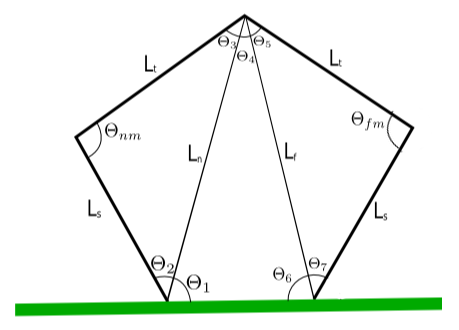
\includegraphics[width=0.7\textwidth]{../figures/bothbound_model.png}
%% \end{figure}

\section{Derivation of bothbound tail coordinates}

\begin{align*}
  \theta_1 &= \cos^{-1}\left(\frac{X_{fm}-X_{nm}}{L}\right)\\
  \theta_2 &= \cos^{-1}\left(\frac{L}{2L_t}\right)\\
  L &= \sqrt{(X_{fm}-X_{nm})^2+(Y_{fm}-Y_{nm})^2}\\
\end{align*}

\subsection{$X_t$}
\begin{align*}
  X_t &= X_{nm} + L_t\cos(\theta_1 \pm \theta_2)\\
  &= X_{nm} + L_t\cos\left(\cos^{-1}\left(\frac{X_{fm}-X_{nm}}{L}\right) \pm \cos^{-1}\left(\frac{L}{2L_t}\right) \right)
  \hspace*{1in} \cos\Big(cos^{-1}(a)\pm cos^{-1}(b)\Big) = ab \mp \sqrt{1-a^2}\sqrt{1-b^2}\\
  &= X_{nm} + L_t\left(\frac{X_{fm}-X_{nm}}{2L_t} \mp \sqrt{1 - \frac{\left(X_{fm}-X_{nm}\right)^2}{L^2}}\sqrt{1 - \frac{L^2}{4L_t^2}}\right)\\
  &= \frac{X_{fm}+X_{nm}}{2} \mp \frac{1}{2}\sqrt{1 - \frac{\left(X_{fm}-X_{nm}\right)^2}{L^2}}\sqrt{4L_t - L^2}\\
  &= \frac{X_{fm}+X_{nm}}{2} \mp \frac{1}{2L}\sqrt{L^2 - \left(X_{fm}-X_{nm}\right)^2}\sqrt{4L_t - L^2}\\
  &= \frac{X_{fm}+X_{nm}}{2} \mp \frac{1}{2}\sqrt{(Y_{fm}-Y_{nm})^2}\sqrt{\frac{4L_t}{L^2} - 1}\\
  &= \frac{X_{fm}+X_{nm}}{2} \mp \frac{Y_{fm}-Y_{nm}}{2L}\sqrt{\frac{4L_t^2}{\left(X_{fm}-X_{nm}\right)^2 + \left(Y_{fm}-Y_{nm}\right)^2} -1}\\
  &= \frac{X_{fm}+X_{nm}}{2} \mp \frac{Y_{fm}-Y_{nm}}{2}\sqrt{\frac{4L_t^2}{X_{fm}^2 + X_{nm}^2 + Y_{fm}^2 + Y_{nm}^2 -2X_{fm}X_{nm} -2Y_{fm}Y_{nm}} -1}\\
  &= \frac{B + L_s\cos(\theta_{fb}) + L_s\cos(\theta_{nb})}{2} \mp \frac{L_s\sin(\theta_{fb})-L_s\sin(\theta_{nb})}{2} * \\
  &\sqrt{\frac{4L_t^2}{B^2 + L_s^2\cos^2(\theta_{fb}) + 2BL_s\cos(\theta_{fb}) + L_s^2\cos^2(\theta_{nb}) + L_s^2\sin^2(\theta_{fb}) + L_s^2\sin^2(\theta_{nb}) -2(B + L_s\cos(\theta_{fb}))(L_s\cos(\theta_{nb})) -2L_s^2\sin(\theta_{fb})\sin(\theta_{nb})} -1}\\\\
  &= \frac{B + L_s\cos(\theta_{fb}) + L_s\cos(\theta_{nb})}{2} \mp \frac{L_s\sin(\theta_{fb})-L_s\sin(\theta_{nb})}{2} * \\
  &\sqrt{\frac{4L_t^2}{2L_s^2 + B^2 + 2BL_s\cos(\theta_{fb}) - 2BL_s\cos(\theta_{nb}) - 2L_s^2\cos(\theta_{fb})\cos(\theta_{nb}) - 2L_s^2\sin(\theta_{fb})\sin(\theta_{nb})} -1}\\\\
  &= \frac{B + L_s\cos(\theta_{fb}) + L_s\cos(\theta_{nb})}{2} \mp \frac{L_s\sin(\theta_{fb})-L_s\sin(\theta_{nb})}{2}\sqrt{\frac{4L_t^2}{2L_s^2 + B^2 + 2BL_s\cos(\theta_{fb}) - 2BL_s\cos(\theta_{nb}) - 2L_s^2\cos(\theta_{fb} - \theta_{nb})} -1}\\
\end{align*}

\subsection{$Y_t$}
\begin{align*}
  Y_t &= Y_{nm} + L_t\sin(\theta_1 \pm \theta_2)\\
  &= Y_{nm} + L_t\sin\left(\cos^{-1}\left(\frac{X_{fm}-X_{nm}}{L}\right) \pm \cos^{-1}\left(\frac{L}{2L_t}\right) \right)
  \hspace*{1in} \sin\Big(cos^{-1}(a)\pm cos^{-1}(b)\Big) = \sqrt{1-a^2}b\pm a\sqrt{1-b^2}\\
  &= Y_{nm} + L_t\left(\frac{L}{2L_t}\sqrt{1 - \frac{\left(X_{fm}-X_{nm}\right)^2}{L^2}} \pm \frac{X_{fm}-X_{nm}}{L}\sqrt{1 - \frac{L^2}{4L^2_t}}\right)\\
  &= Y_{nm} + \frac{L}{2}\sqrt{1 - \frac{\left(X_{fm}-X_{nm}\right)^2}{L^2}} \pm \frac{X_{fm}-X_{nm}}{2L}\sqrt{4L_t^2 - L^2}\\
  &= Y_{nm} + \frac{1}{2}\sqrt{L^2 - \left(X_{fm}-X_{nm}\right)^2} \pm \frac{X_{fm}-X_{nm}}{2}\sqrt{\frac{4L_t^2}{L^2} - 1}\\
  &= Y_{nm} + \frac{1}{2}\sqrt{\left(Y_{fm}-Y_{nm}\right)^2} \pm \frac{X_{fm}-X_{nm}}{2}\sqrt{\frac{4L_t^2}{\left(X_{fm}-X_{nm}\right)^2 + \left(Y_{fm}-Y_{nm}\right)^2} - 1}\\
  &= \frac{Y_{fm} + Y_{nm}}{2} \pm \frac{X_{fm}-X_{nm}}{2}\sqrt{\frac{4L_t^2}{\left(X_{fm}-X_{nm}\right)^2 + \left(Y_{fm}-Y_{nm}\right)^2} - 1}\\
  &= \frac{Y_{fm} + Y_{nm}}{2} \pm \frac{X_{fm}-X_{nm}}{2}\sqrt{\frac{4L_t^2}{X_{fm}^2 + X_{nm}^2 + Y_{fm}^2 + Y_{nm}^2 -2X_{fm}X_{nm} -2Y_{fm}Y_{nm}} - 1}\\
  &= \frac{L_s\sin(\theta_{fb}) + L_s\sin(\theta_{nb})}{2} \pm \frac{B + L_s\cos(\theta_{fb}) - L_s\cos(\theta_{nb})}{2} *\\
  &\sqrt{\frac{4L_t^2}{B^2 + L_s^2\cos^2(\theta_{fb}) + BL_s\cos(\theta_{fb}) + L_s^2\cos^2(\theta_{nb}) + L_s^2\sin^2(\theta_{fb}) + L_s^2\sin^2(\theta_{nb}) -2(B + L_s\cos(\theta_{fb}))L_s\cos(\theta_{nb}) -2L_s^2\sin(\theta_{fb})\sin(\theta_{nb})} - 1}\\\\
  &= \frac{L_s\sin(\theta_{fb}) + L_s\sin(\theta_{nb})}{2} \pm \frac{B + L_s\cos(\theta_{fb}) - L_s\cos(\theta_{nb})}{2} *\\
  &\sqrt{\frac{4L_t^2}{2L_s^2 + B^2 + BL_s\cos(\theta_{fb}) -2BL_s\cos(\theta_{nb}) - 2L_s^2\cos(\theta_{fb})\cos(\theta_{nb}) - 2L_s^2\sin(\theta_{fb})\sin(\theta_{nb})} - 1}\\\\
  &= \frac{L_s\sin(\theta_{fb}) + L_s\sin(\theta_{nb})}{2} \pm \frac{B + L_s\cos(\theta_{fb}) - L_s\cos(\theta_{nb})}{2}\sqrt{\frac{4L_t^2}{2L_s^2 + B^2 + BL_s\cos(\theta_{fb}) -2BL_s\cos(\theta_{nb}) - 2L_s^2\cos(\theta_{fb} - \theta_{nb})} - 1}\\
\end{align*}

\section{Cartesian from Angular Coordinates}
This section lays out the definitions of the coordinates of the bothbound Dynein model.\\
\begin{align}
  X_{nb} &= 0\\
  X_{nm} &= L_s\cos(\theta_{nb})\\
  X_{t}  &= \frac{B + L_s\cos(\theta_{fb}) + L_s\cos(\theta_{nb})}{2} \mp \frac{L_s\sin(\theta_{fb})-L_s\sin(\theta_{nb})}{2}\sqrt{\frac{4L_t^2}{2L_s^2 + B^2 + 2BL_s\cos(\theta_{fb}) - 2BL_s\cos(\theta_{nb}) - 2L_s^2\cos(\theta_{fb} - \theta_{nb})} -1}\\
  X_{fm} &= B + L_s\cos(\theta_{fb})\\
  X_{fb} &= B \\
\end{align}

\begin{align}
  Y_{nb} &= 0 \\
  Y_{nm} &= L_s\sin(\theta_{nb})\\
  Y_{t}  &= \frac{L_s\sin(\theta_{fb}) + L_s\sin(\theta_{nb})}{2} \pm \frac{B + L_s\cos(\theta_{fb}) - L_s\cos(\theta_{nb})}{2}\sqrt{\frac{4L_t^2}{2L_s^2 + B^2 + BL_s\cos(\theta_{fb}) -2BL_s\cos(\theta_{nb}) - 2L_s^2\cos(\theta_{fb} - \theta_{nb})} - 1}\\
  Y_{fm} &= L_s\sin(\theta_{fb})\\
  Y_{fb} &= 0\\
\end{align}

\section{Cartesian Velocities}
This section shows the velocity definitions. \\
\begin{align}
  \dot{X}_{nb} &= 0 \\
  \dot{X}_{nm} &= -L_s\sin(\theta_{nb})\dot{\theta}_{nb}\\
  \dot{X}_{t } &= \frac{-L_s\sin(\theta_{fb})\dot{\theta}_{fb} + -L_s\sin(\theta_{nb})\dot{\theta}_{nb}}{2} \mp \frac{L_s\cos(\theta_{fb})\dot{\theta}_{fb} - L_s\cos(\theta_{nb})\dot{\theta}_{nb}}{2}\sqrt{\frac{4L_t^2}{2L_s^2 + B^2 + 2BL_s\cos(\theta_{fb}) - 2BL_s\cos(\theta_{nb}) - 2L_s^2\cos(\theta_{fb} - \theta_{nb})} -1}\\
  &\pm \frac{L_s\sin(\theta_{fb})-L_s\sin(\theta_{nb})}{2}\frac{\frac{-4L_t^2}{\left(2L_s^2 + B^2 + 2BL_s\cos(\theta_{fb}) - 2BL_s\cos(\theta_{nb}) - 2L_s^2\cos(\theta_{fb} - \theta_{nb})\right)^2} \left(-2BL_s\sin(\theta_{fb})\dot{\theta}_{fb} + 2BL_s\sin(\theta_{nb})\dot{\theta}_{nb} + 2L_s^2\sin(\theta_{fb} - \theta_{nb})(\dot{\theta}_{fb}+\dot{\theta}_{nb})\right)}{2\sqrt{\frac{4L_t^2}{2L_s^2 + B^2 + 2BL_s\cos(\theta_{fb}) - 2BL_s\cos(\theta_{nb}) - 2L_s^2\cos(\theta_{fb} - \theta_{nb})} -1}}\\
  \dot{X}_{fm} &= -L_s\sin(\theta_{fb})\dot{\theta}_{fb}\\
  \dot{X}_{fb} &= 0
\end{align}

\begin{align}                                                                  
  \dot{Y}_{nb} &= 0 \\                                 
  \dot{Y}_{nm} &= L_s\cos(\theta_{nb})\dot{\theta}_{nb}\\
  \dot{Y}_{t}  &= \frac{L_s\cos(\theta_{fb})\dot{\theta}_{fb} + L_s\cos(\theta_{nb})\dot{\theta}_{nb}}{2}\pm \frac{-L_s\sin(\theta_{fb})\dot{\theta}_{fb} + L_s\sin(\theta_{nb})\dot{\theta}_{nb}}{2}\sqrt{\frac{4L_t^2}{2L_s^2 + B^2 + BL_s\cos(\theta_{fb}) -2BL_s\cos(\theta_{nb}) - 2L_s^2\cos(\theta_{fb} - \theta_{nb})} - 1} \\
 &\pm \frac{B + L_s\cos(\theta_{fb}) - L_s\cos(\theta_{nb})}{2}\frac{\frac{-4L_t^2}{\left(2L_s^2 + B^2 + BL_s\cos(\theta_{fb}) -2BL_s\cos(\theta_{nb}) - 2L_s^2\cos(\theta_{fb} - \theta_{nb})\right)^2}-BL_s\sin(\theta_{fb})\dot{\theta}_{fb} + 2BL_s\sin(\theta_{nb})\dot{\theta}_{nb} + 2L_s^2\sin(\theta_{fb} - \theta_{nb})(\dot{\theta}_{fb}+\dot{\theta}_{nb})}{2\sqrt{\frac{4L_t^2}{2L_s^2 + B^2 + BL_s\cos(\theta_{fb}) -2BL_s\cos(\theta_{nb}) - 2L_s^2\cos(\theta_{fb} - \theta_{nb})} - 1}}\\
  \dot{Y}_{fm} &= L_s\cos(\theta_{fb})\dot{\theta}_{fb}\\
  \dot{Y}_{fb} &= 0 \\
\end{align}

\begin{twocolumn}
\section{Notes on physical parameters}

Stoke's Law states that the relationship between viscosity, force, and
velocity for a spherical particle is given by:
\begin{align}
  \mathbf{v} &= \frac{\mathbf{F}}{6\pi \mu R}
\end{align}
where $\mu$ is the viscosity of the fluid, and $R$ is the radius of
the particle.  Thus in our terminology:
\begin{align}
  \gamma &= 6\pi \mu R.
\end{align}
Note that the viscosity of water is temperature-dependent and around
0.7~mPa~s at body temperature.  However, the viscosity of cytoplasm
may be rather different, and will of course depend on length scale.
But for our purposes we can probably get away with this value.

The random force $\mathbf{R}(t)$ should have a Gaussian distribution
with variance~1, but then be divided by $\sqrt{\Delta t}$.  Thus, the
smaller the time step, the larger the random force we will apply.  We
can understand this in the backwards direction.  When we observe a
larger time step, the ``random force'' results from many smaller
random forces added together, and these smaller forces often cancel,
leading to this reduction in the total force over that time period.

Finally, we will need estimates for the radii of each domain (to go
into the $\gamma$ parameter, the equilibrium angles for each hinge, and
the spring constants for each hinge.  The first two we can estimate
from the structure of dynein.  The third will require a rough guess.
We can get a ball-park guess by deciding how much we want the angle to
fluctuate (e.g. $\ll \pi$ for each angle!), and then take our spring
constant to be $kT$ divided by that anglular fluctuation squared.

\end{twocolumn}

\end{document}


























